\documentclass[11pt,letterpaper]{article}

\usepackage[top=1in, 
left=1in, 
right=1in, 
bottom=1in]{geometry}
\usepackage{setspace}
\usepackage{titling}
\newcommand{\subtitle}[1]{%
	\posttitle{%
		\par\end{center}
	\begin{center}\large#1\end{center}
	\vskip0.5em}%
}

\usepackage{lmodern}
\usepackage{amssymb,amsmath,bm,bbm}
\renewcommand{\familydefault}{\sfdefault}

\DeclareMathOperator*{\argmax}{argmax}


\usepackage{booktabs,caption,subcaption,threeparttable}
\usepackage{graphicx}

\usepackage[hyperfootnotes=false, 
colorlinks=true, 
allcolors=black]{hyperref}

\usepackage[backend=biber, 
authordate, 
maxcitenames=2, 
uniquename=false, 
uniquelist=false, 
url=false, 
doi=false, 
isbn=false]{biblatex-chicago}
\addbibresource{refs.bib}
\usepackage{bibentry}
\setlength{\bibhang}{0pt}

\begin{document}

\title{Maximum Likelihood Estimation}
\subtitle{Topics in Advanced Econometrics (ResEcon 703)\vspace{-2ex}}
\author{Matt Woerman\\Resource Economics, UMass Amherst}
%\date{}  % Toggle commenting to test
\date{\vspace{-5ex}}

\maketitle

\section{Overview of maximum likelihood estimation}

Maximum likelihood (ML) estimation\footnote{Maximum likelihood estimation is often abbreviated as MLE, but so too is the maximum likelihood estimator. To avoid confusion, I will use ML as an abbreviation for the maximum likelihood method, and I will use MLE as an abbreviation for the maximum likelihood estimator. This could instead create confusion between maximum likelihood and machine learning, which is also commonly abbreviated as ML. But we will not cover machine learning in this course, so ML will always refer to maximum likelihood.} is one of the most common estimation methods in structural econometrics. A primary reason that ML is often used in structural estimation is that it is more flexible than other methods, such as ordinary least squares (OLS) regression. In particular, ML can estimate the parameters of a nonlinear model, which is common in structural econometric models. ML can be used for simpler models as well and, in fact, OLS is a special case of ML. This flexibility, however, requires stronger distributional assumptions than OLS. When these assumptions hold, the maximum likelihood estimator (MLE) is consistent and efficient. But if these assumptions are invalid, the interpretation of the MLE is less clear. 

\subsection{Intuition of maximum likelihood estimation}

The basic intuition of maximum likelihood estimation is best illustrated through an example. Suppose we have five random draws from a normal distribution, $\bm{y} = \{48.7, 50.9, 48.8, 50.6, 48.8\}$, but we do not know which normal distribution, $\mathcal{N}(\mu, \sigma^2)$. In other words, we know these random draws come from a normal distribution but we do not know the mean, $\mu$, or the variance, $\sigma^2$, of the specific normal distribution that generated these random draws. \\

\noindent Consider two possible candidates for the normal distribution, $\mathcal{N}(0, 1)$ and $\mathcal{N}(50, 1)$. What is the likelihood\footnote{I use the term likelihood rather than probability because, from a frequentist perspective, the true underlying distribution is already determined---even though we do not know what it is---so its probability has no useful meaning.} that these random draws, $\bm{y} = \{48.7, 50.9, 48.8, 50.6, 48.8\}$, came from a standard normal distribution, $\mathcal{N}(0, 1)$? Practically zero. What is the likelihood that these random draws came, instead, from a normal distribution with a mean of 50, $\mathcal{N}(50, 1)$? Much more likely! Given these data, we would say that the distribution $\mathcal{N}(50, 1)$ has a greater likelihood than $\mathcal{N}(0, 1)$ of having generated these data. \\ 

\noindent This simple example illustrates the basic intuition of maximum likelihood estimation and the maximum likelihood estimator---we want to find the set of parameters that maximize the likelihood of having generated that we actually observe.

\subsection{Probability density function and likelihood function}

Before formally describing ML, it is helpful to have one key statistical object in mind: the probability density function (PDF).\footnote{Or the probability mass function (PMF) in the case of a discrete distribution.} The PDF is a mathematical expression that gives us the relative likelihood that a random variable would take a particular value. The PDF for a random variable $y$ is often denoted $f(y \mid \bm{\theta})$, where $\bm{\theta}$ is the set of parameters that describe the specific distribution of the random variable. For example, in the case of a normal distribution, the parameters are $\bm{\theta} = \left( \mu, \sigma^2 \right)$, and the PDF is
$$f(y \mid \mu, \sigma^2) = \frac{1}{\sqrt{2 \pi \sigma^2}} e^{\frac{-(y - \mu)^2}{2 \sigma^2}}$$
A graphical representation of the standard normal PDF, or $f(y \mid 0, 1)$ is plotted in Figure \ref{fig:norm_pdf}.

\begin{figure}[htbp]
  \caption{Probability density function of a standard normal distribution}
  \label{fig:norm_pdf}
  \centering
  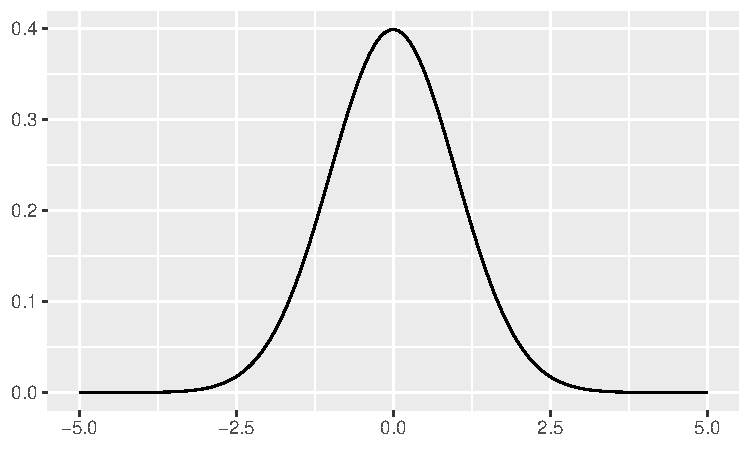
\includegraphics[width=0.8\textwidth]{norm_pdf.pdf}
\end{figure}

\noindent The implicit assumption in a PDF is that the parameters are defined and the random variable is yet to be determined. In econometrics, however, the opposite is almost always true---we have the resulting data of the data-generating process, but we do not know and want to estimate the parameters that gave rise to those data. In this case, we can use the same mathematical expression to give the likelihood that a particular set of parameter values would have generated the sample that we observe. We call this the likelihood function and denote it as $L(\bm{\theta} \mid \bm{y})$. For example, in the case of a normal distribution, the likelihood function of the parameters $\bm{\theta} = \left( \mu, \sigma^2 \right)$ for a single random draw, $y$, is
$$L(\mu, \sigma^2 \mid y) = \frac{1}{\sqrt{2 \pi \sigma^2}} e^{\frac{-(y - \mu)^2}{2 \sigma^2}}$$
Note that the right-hand side of this expression is the same as the PDF. The only difference is conceptual---which parts of the expression are taken to be known and which parts are taken to be unknown.

\section{Maximum likelihood estimator}

Maximum likelihood estimation requires a distributional assumption about the data-generating process of the data we observe. We assume the probability density function for a random variable, $y$, conditioned on a set of parameters, $\bm{\theta}$, is $f(y \mid \bm{\theta})$.\footnote{We could generalize to a random vector, $\bm{y}$, with joint density $f(\bm{y} \mid \bm{\theta})$, but the simpler assumption of a single random variable will be sufficient for this course.} This PDF identifies the data-generating process that underlies an observed sample of data and provides a mathematical description of the data that the process will produce. Note that by assuming $y$ has PDF $f(y \mid \bm{\theta})$, we are making an assumption about the density of $y$, not just its expectation or variance. \\

\noindent The joint density of $n$ independent and identically distributed (i.i.d.) random variables, each with density $f(y \mid \bm{\theta})$, is
\begin{align*}
  f(y_1, \ldots, y_n \mid \bm{\theta}) & = \prod_{i = 1}^n f(y_i \mid \bm{\theta})
  \intertext{The conditioning in this joint density suggests that the parameters are known and the data are unknown, but, as described above, this is rarely the case in econometrics. Instead, we almost always have data and want to know the parameters of the data-generating process. We simply switch the conditioning and define the likelihood function as a function of the unknown parameters, $\bm{\theta}$, conditioned on the data we observe, $\bm{y}$:}
  L(\bm{\theta} \mid \bm{y}) & = \prod_{i = 1}^n f(y_i \mid \bm{\theta})
  \intertext{It will often be easier to work with the log of the likelihood function, or the log-likelihood function:}
  \ln L(\bm{\theta} \mid \bm{y}) & = \sum_{i = 1}^n \ln f(y_i \mid \bm{\theta})
\end{align*}
Log is a monotonic transformation, so finding the greatest log-likelihood is equivalent to finding the greatest likelihood, but it is often easier to use the log-likelihood function because it involves taking a sum rather than a product. \\

\noindent The maximum likelihood estimator, which we denote $\widehat{\bm{\theta}}$, is the set of parameters that maximizes the likelihood function and is equivalent to the set of parameters that maximizes the log-likelihood function:
\begin{align*}
  \widehat{\bm{\theta}} & = \argmax_{\bm{\theta}} L(\bm{\theta} \mid \bm{y}) \\
  \widehat{\bm{\theta}} & = \argmax_{\bm{\theta}} \ln L(\bm{\theta} \mid \bm{y})
\end{align*}
In words, the MLE is the set of parameters that maximizes the likelihood of having generated that data that we actually observe. A necessary condition for maximizing the log-likelihood function is that, at the MLE, the derivative of the log-likelihood function with respect to each parameter must equal zero:
$$\frac{\partial \ln L(\bm{\theta} \mid \bm{y})}{\partial \bm{\theta}} = \bm{0}$$
In some cases, these first-order conditions yield closed-form expressions for the MLE. For more complex estimation, numerical maximization is required to find the MLE. \\

\noindent So far, we have only described having data, $\bm{y}$, that are conditional on parameters, $\bm{\theta}$. In most cases, however, we model some outcome data, $\bm{y}$, as a function of both parameters, $\bm{\theta}$, and other data, $\bm{X}$. When $y$ is also a function of data, $\bm{x}$, we need to define its conditional PDF, $f(y \mid \bm{x}, \bm{\theta})$. In almost all cases,\footnote{The exception is if the conditional PDF of $y$, $f(y \mid \bm{x}, \bm{\theta})$, and the joint PDF of $\bm{x}$, $g(\bm{x} \mid \bm{\delta})$, depend on some common parameters. So long as these data-generating processes depend on different parameters, we can effectively ignore the data-generating process of $\bm{x}$ and consider only the conditional PDF of $y$.} we can simply simply substitute this conditional PDF in place of the PDF in previous expressions. For example, when $y$ depends on both $\bm{x}$ and $\bm{\theta}$, the likelihood and log-likelihood functions are
\begin{align*}
  L(\bm{\theta} \mid \bm{y}, \bm{X}) & = \prod_{i = 1}^n f(y_i \mid \bm{x}_i, \bm{\theta}) \\
  \ln L(\bm{\theta} \mid \bm{y}, \bm{X}) & = \sum_{i = 1}^n \ln f(y_i \mid \bm{x}_i, \bm{\theta})
\end{align*}
These functions are technically the conditional likelihood function and the conditional log-likelihood, but this conditioning is so common that the ``conditional'' terminology is often dropped for convenience.

\section{Examples of maximum likelihood estimation}

\subsection{Poisson distribution}

Suppose we have ten random draws, $\bm{y}$, from a Poisson distribution:
$$\bm{y} = \{ 2, 0, 1, 2, 2, 2, 0, 2, 1, 1 \}$$
with the probability mass function (PMF)
$$f(y \mid \lambda) = \frac{e^{-\lambda} \lambda^y }{y!}$$
Although we know these data come from a Poisson distribution, we do not know which Poisson distribution; that is, we do not know the $\lambda$ parameter that defines the distribution. Figure \ref{fig:pois_pmf} plots the Poisson PMF for three of the possible values of $\lambda$. We can use ML to estimate the value of the $\lambda$ parameter that maximizes the likelihood of generating the data we observe. \\

\begin{figure}[htbp]
  \caption{Probability mass function of Poisson distributions}
  \label{fig:pois_pmf}
  \begin{subfigure}{.33\textwidth}
    \centering
    \caption*{$f(y \mid 1)$}
    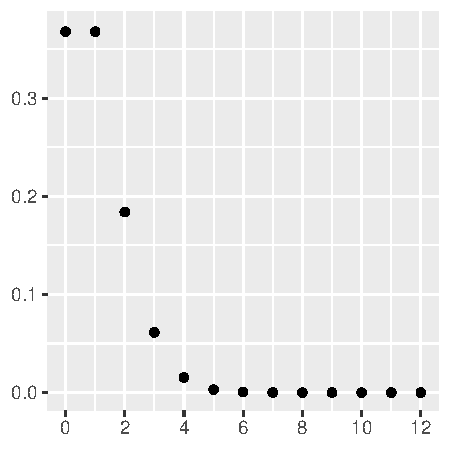
\includegraphics[width=\linewidth]{pois_1_pmf.pdf}
  \end{subfigure}%
  \begin{subfigure}{.33\textwidth}
    \centering
    \caption*{$f(y \mid 3)$}
    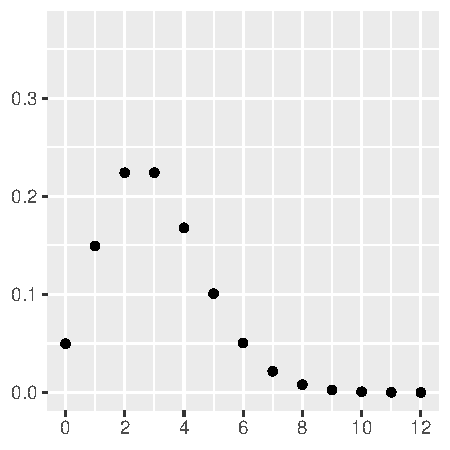
\includegraphics[width=\linewidth]{pois_3_pmf.pdf}
  \end{subfigure}
  \begin{subfigure}{.33\textwidth}
    \centering
    \caption*{$f(y \mid 5)$}
    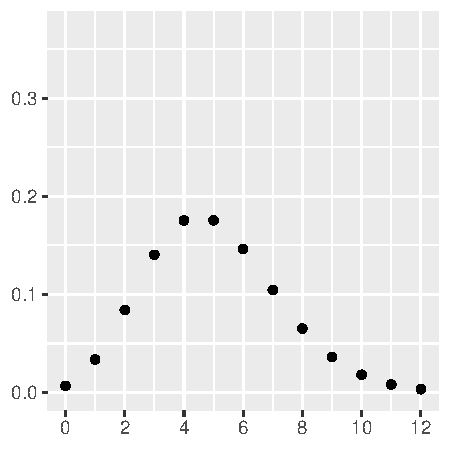
\includegraphics[width=\linewidth]{pois_5_pmf.pdf}
  \end{subfigure}
\end{figure}

\noindent The likelihood function of $\lambda$ conditional on $\bm{y}$ is the product of the PMF for each random draw:
\begin{align*}
  L(\lambda \mid \bm{y}) & = \prod_{i = 1}^n \frac{e^{-\lambda} \lambda^{y_i} }{y_i!} = \frac{e^{-n \lambda} \lambda^{\sum_{i=1}^n y_i}}{\prod_{i = 1}^n y_i!}
  \intertext{The log-likelihood function of $\lambda$ conditional on $\bm{y}$ is simply the log of this likelihood function:}
  \ln L(\lambda \mid \bm{y}) & = -n \lambda + \ln \lambda \sum_{i = 1}^n y_i - \sum_{i = 1}^n \ln (y_i!)
  \intertext{A necessary condition for the MLE is that the derivative of this log-likelihood function with respect to $\lambda$ equals zero. This derivative is}
  \frac{\partial \ln L(\lambda \mid \bm{y})}{\partial \lambda} & = -n + \frac{1}{\lambda} \sum_{i = 1}^n y_i
\end{align*}
Setting this derivative equal to zero and solving for $\lambda$ yields an expression for the MLE, $\widehat{\lambda}$:
$$\frac{\partial \ln L(\lambda \mid \bm{y})}{\partial \lambda} = 0 ~~ \Rightarrow ~~ \widehat{\lambda} = \frac{1}{n} \sum_{i = 1}^n y_i$$
This expression defines the MLE, $\widehat{\lambda}$, as a function of our data. In fact, for the Poisson distribution, the MLE is simply the sample mean of the data. Plugging in our data yields the MLE:
$$\widehat{\lambda} = \frac{1}{n} \sum_{i = 1}^n y_i = 1.3$$
In other words, a $\lambda$ parameter value of $\widehat{\lambda} = 1.3$ is the most likely of all possible $\lambda$ values to have generated the data that we observe, $\bm{y}$. \\

\noindent We can also visualize the likelihood and log-likelihood functions of $\lambda$ conditional on our data. Using the likelihood function above and plugging in our data gives
$$L(\lambda \mid \bm{y}) = \prod_{i = 1}^n \frac{e^{-\lambda} \lambda^{y_i} }{y_i!} = \frac{e^{-n \lambda} \lambda^{\sum_{i=1}^n y_i}}{\prod_{i = 1}^n y_i!} = \frac{e^{-10 \lambda} \lambda^{\sum_{i=1}^n 13}}{32}$$
The left panel of Figure \ref{fig:pois_lll} plots this likelihood function, and we can see this function is maximized at a value of $\widehat{\lambda} = 1.3$. Similarly, using the log-likelihood function above and plugging in our data gives
$$\ln L(\lambda \mid \bm{y}) = -n \lambda + \ln \lambda \sum_{i = 1}^n y_i - \sum_{i = 1}^n \ln (y_i!) = -10 \lambda + 13 \ln \lambda - 3.47$$
The right panel of Figure \ref{fig:pois_lll} plots this log-likelihood function, and we can see this function is also maximized at a value of $\widehat{\lambda} = 1.3$.

\begin{figure}[htbp]
  \caption{Likelihood and log-likelihood functions of Poisson example}
  \label{fig:pois_lll}
  \centering
  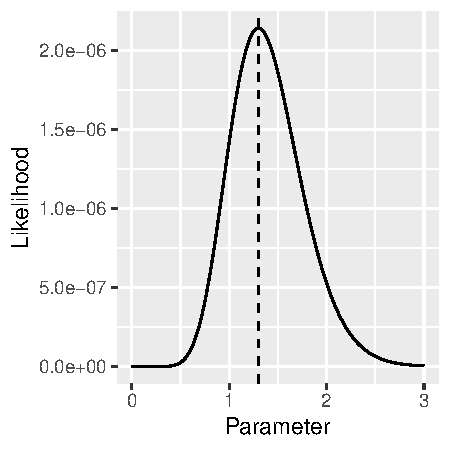
\includegraphics[width=0.49\textwidth]{likelihood.pdf}
  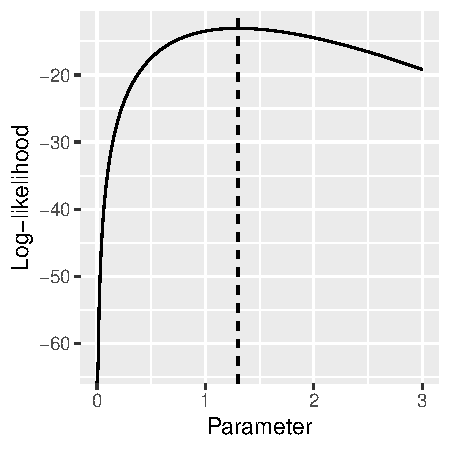
\includegraphics[width=0.49\textwidth]{log_likelihood.pdf}
\end{figure}

\subsection{Normal distribution}

Suppose we have five random draws, $\bm{y}$, from a normal distribution:
$$\bm{y} = \{ 6.08, 5.29, 2.52, 2.94, 5.36 \}$$
with the PDF
$$f(y \mid \mu, \sigma^2) = \frac{1}{\sqrt{2 \pi \sigma^2}} e^{\frac{-(y - \mu)^2}{2 \sigma^2}}$$
Although we know these data come from a normal distribution, we do not know which normal distribution. Note that a normal distribution is defined by two parameters: the mean, $\mu$, and the variance, $\sigma^2$. We can use ML to estimate the values of $\mu$ and $\sigma^2$ that maximize the likelihood of generating the data we observe. \\

\noindent The likelihood function of $\mu$ and $\sigma^2$ conditional on $\bm{y}$ is the product of the PDF for each random draw:
\begin{align*}
  L(\mu, \sigma^2 \mid \bm{y}) & = \prod_{i = 1}^n f(y_i \mid \mu, \sigma^2) = \left( \frac{1}{\sqrt{2 \pi \sigma^2}} \right)^n e^{-\frac{1}{2 \sigma^2} \sum_{i = 1}^n (y_i - \mu)^2}
  \intertext{The log-likelihood function of $\mu$ and $\sigma^2$ conditional on $\bm{y}$ is simply the log of this likelihood function:}
  \ln L(\mu, \sigma^2 \mid \bm{y}) & = -\frac{n}{2} \ln 2 \pi - \frac{n}{2} \ln \sigma^2 - \frac{1}{2 \sigma^2} \sum_{i = 1}^n (y_i - \mu)^2
\end{align*}
A necessary condition for the MLE is that the derivative of this log-likelihood function with respect to each parameter equals zero. Note that there are two parameters, so we have first-order conditions for each of these two parameters. These derivatives are
\begin{align*}
  \frac{\partial \ln L(\mu, \sigma^2 \mid \bm{y})}{\partial \mu} & = \frac{1}{\sigma^2} \sum_{i = 1}^n (y_i - \mu) \\
  \frac{\partial \ln L(\mu, \sigma^2 \mid \bm{y})}{\partial \sigma^2} & = - \frac{n}{2 \sigma^2} + \frac{1}{2 \sigma^4} \sum_{i = 1}^n (y_i - \mu)^2
\end{align*}
Setting each of these derivatives equal to zero and solving for each parameter yields an expression for the MLE, $\widehat{\mu}$ and $\widehat{\sigma}^2$:
\begin{align*}
  \frac{\partial \ln L(\mu, \sigma^2 \mid \bm{y})}{\partial \mu} & = 0 ~~ \Rightarrow ~~ \widehat{\mu} = \frac{1}{n} \sum_{i = 1}^n y_i \\
  \frac{\partial \ln L(\mu, \sigma^2 \mid \bm{y})}{\partial \sigma^2} & = 0 ~~ \Rightarrow ~~ \widehat{\sigma}^2 = \frac{1}{n} \sum_{i = 1}^n (y_i - \widehat{\mu})^2
\end{align*}
These expressions define the MLE, $\widehat{\mu}$ and $\widehat{\sigma}^2$, as a function of our data. In fact, for the normal distribution, the MLE of the mean parameter is simply the sample mean of the data and the MLE of the variance parameter is simply the sample variance of the data. Plugging in our data yields the MLE:
\begin{align*}
  \widehat{\mu} & = \frac{1}{n} \sum_{i = 1}^n y_i = 4.44 \\
  \widehat{\sigma}^2 & = \frac{1}{n} \sum_{i = 1}^n (y_i - \widehat{\mu})^2 = 2.04
\end{align*}
In other words, parameter values of $\widehat{\mu} = 4.44$ and $\widehat{\sigma}^2 = 2.04$ are the most likely of all possible combinations of $\mu$ and $\sigma^2$ values to have generated the data that we observe, $\bm{y}$.

\subsection{Ordinary least squares regression}

In the previous two examples, we estimated the parameters that maximize the likelihood of generating the data that we observe. In most econometric applications, however, we model some outcome data, $\bm{y}$, as a function of both parameters, $\bm{\theta}$, and other data $\bm{X}$. An example is a simple ordinary least squares (OLS) regression:
$$y_i = \beta_0 + \beta_1 x_i + \varepsilon_i$$
If we make a distributional assumption about the error term, $\varepsilon_i$, we will have the distribution of $y_i$ conditional on $x_i$ parameters, $f(y_i \mid x_i, \bm{\theta})$. We can then use this conditional distribution of $y_i$ to maximize the likelihood of the parameters and find the MLE, $\widehat{\bm{\theta}}$. Note that OLS is a special case of ML, so the MLE will be equivalent to the traditional OLS estimator, but we will find those values in a different way. \\

\noindent The standard distributional assumption in an OLS regression is that the error term is mean-zero with variance of $\sigma^2$:
$$\varepsilon_i \sim \mathcal{N}(0, \sigma^2)$$
Then $y_i$ will have a conditional distribution---conditional on the value of $x_i$---that is normal, but with a mean of $\beta_0 + \beta_1 x_i$ and a variance of $\sigma^2$:
$$y_i \mid x_i \sim \mathcal{N}(\beta_0 + \beta_1 x_i, \sigma^2)$$
The conditional probability density function of $y_i$ is
$$f(y_i \mid x_i, \beta_0, \beta_1, \sigma^2) = \frac{1}{\sqrt{2 \pi \sigma^2}} e^{\frac{-(y_i - \beta_0 - \beta_1 x_i)^2}{2 \sigma^2}}$$

\noindent The conditional likelihood function of $\beta_0$, $\beta_1$, and $\sigma^2$ conditional on both $\bm{y}$ and $\bm{x}$ is the product of the conditional PDF for each $y_i$ value:
\begin{align*}
  L(\beta_0, \beta_1, \sigma^2 \mid \bm{y}, \bm{x}) & = \prod_{i = 1}^n f(y_i \mid x_i, \beta_0, \beta_1, \sigma^2) = \left( \frac{1}{\sqrt{2 \pi \sigma^2}} \right)^n e^{-\frac{1}{2 \sigma^2} \sum_{i = 1}^n (y_i - \beta_0 - \beta_1 x_i)^2}
  \intertext{The conditional log-likelihood function of $\beta_0$, $\beta_1$, and $\sigma^2$ conditional on $\bm{y}$ and $\bm{x}$ is simply the log of this likelihood function:}
  \ln L(\beta_0, \beta_1, \sigma^2 \mid \bm{y}, \bm{x}) & = -\frac{n}{2} \ln 2 \pi - \frac{n}{2} \ln \sigma^2 - \frac{1}{2 \sigma^2} \sum_{i = 1}^n (y_i - \beta_0 - \beta_1 x_i)^2
\end{align*}
A necessary condition for the MLE is that the derivative of this log-likelihood function with respect to each parameter equals zero. Note that there are three parameters that fully describe the conditional distribution of $y_i$, so we have first-order conditions for each of these three parameters. These derivatives are
\begin{align*}
  \frac{\partial \ln L(\beta_0, \beta_1, \sigma^2 \mid \bm{y}, \bm{x})}{\partial \beta_0} & = \frac{1}{\sigma^2} \sum_{i = 1}^n (y_i - \beta_0 - \beta_1 x_i) \\
  \frac{\partial \ln L(\beta_0, \beta_1, \sigma^2 \mid \bm{y}, \bm{x})}{\partial \beta_1} & = \frac{1}{\sigma^2} \sum_{i = 1}^n x_i (y_i - \beta_0 - \beta_1 x_i) \\
  \frac{\partial \ln L(\beta_0, \beta_1, \sigma^2 \mid \bm{y}, \bm{x})}{\partial \sigma^2} & = - \frac{n}{2 \sigma^2} + \frac{1}{2 \sigma^4} \sum_{i = 1}^n (y_i - \beta_0 - \beta_1 x_i)^2
\end{align*}
Setting each of these derivatives equal to zero and solving for each parameter yields an expression for the MLE, $\widehat{\beta_0}$, $\widehat{\beta_1}$, and $\widehat{\sigma}^2$:
\begin{align*}
  \frac{\partial \ln L(\beta_0, \beta_1, \sigma^2 \mid \bm{y}, \bm{x})}{\partial \beta_0} & = 0 ~~ \Rightarrow ~~ \widehat{\beta}_0 = \bar{y} - \widehat{\beta}_1 \bar{x} \\
  \frac{\partial \ln L(\beta_0, \beta_1, \sigma^2 \mid \bm{y}, \bm{x})}{\partial \beta_1} & = 0 ~~ \Rightarrow ~~ \widehat{\beta}_1 = \frac{\sum_{i = 1}^n (x_i - \bar{x})(y_i - \bar{y})}{\sum_{i = 1}^n (x_i - \bar{x})^2} \\
  \frac{\partial \ln L(\beta_0, \beta_1, \sigma^2 \mid \bm{y}, \bm{x})}{\partial \sigma^2} & = 0 ~~ \Rightarrow ~~ \widehat{\sigma}^2 = \frac{1}{n} \sum_{i = 1}^n (y_i - \widehat{\beta}_0 - \widehat{\beta}_1 x_i)^2
\end{align*}
where $\bar{x}$ and $\bar{y}$ are the sample means of $\bm{x}$ and $\bm{y}$, respectively
\begin{align*}
  \bar{x} & = \frac{1}{n} \sum_{i = 1}^n x_i \\
  \bar{y} & = \frac{1}{n} \sum_{i = 1}^n y_i
\end{align*}
This MLE for an OLS regression is equivalent to the traditional OLS estimator. Thus, we can interpret OLS parameters as not only minimizing the sum or squared error but also maximizing the likelihood of generating the data we observe.

\section{Properties of the maximum likelihood estimator}

Maximum likelihood is commonly used in structural estimation because the MLE has desirable asymptotic properties. When the required distributional assumption is valid and certain regularity conditions are met, the MLE is consistent, asymptotically normal, asymptotically efficient, and invariant to transformations. \\

\noindent The required regularity conditions are:
\begin{enumerate}
  \item The first three derivatives of $\ln f(y_i \mid \bm{\theta})$ with respect to $\bm{\theta}$ are continuous and finite for almost all $y_i$ and for all $\bm{\theta}$.
  \item The conditions necessary to obtain the expectations of the first and second derivatives of ${\ln f(y_i \mid \bm{\theta})}$ are met.
  \item For all values of $\bm{\theta}$, $\left\vert \frac{\partial^3 \ln f(y_i \mid \bm{\theta})}{\partial \theta_j \partial \theta_k \partial \theta_l} \right\vert$ is less than a function that has a finite expectation.
\end{enumerate}
These regularity conditions ensure that the log-likelihood function meets some basic requirements for being ``well-behaved'' so that its moments and derivatives exist. \\

\noindent When these regularity conditions are met and the distributional assumption is valid, the MLE has the properties listed above, which are described in more detail below.\footnote{For the proofs of these properties, see \fullcite{greeneEconometricAnalysis2018}.} In this and future sections, $\widehat{\bm{\theta}}$ denotes the MLE, $\bm{\theta}_0$ denotes the true values of the parameters, $\bm{\theta}$ denotes any arbitrary set of parameters, and $E_0[\cdot]$ denotes the expectation based on the true parameters values. 

\paragraph{Consistency} The MLE converges in probability to the true parameters values:
$$\widehat{\bm{\theta}} \overset{p}{\rightarrow} \bm{\theta}_0$$
In words, as the sample size increases to infinity, the MLE becomes vanishingly close to the true parameter values.

\paragraph{Asymptotic normality} The MLE is asymptotically normal with a mean at the true parameter values and known variance:
$$\widehat{\bm{\theta}} \overset{a}{\sim} \mathcal{N} \left( \bm{\theta}_0, \left\{ -E_0 \left[ \frac{\partial^2 \ln L(\bm{\theta}_0)}{\partial \bm{\theta}_0 \partial \bm{\theta}_0'} \right] \right\}^{-1} \right)$$
In words, the asymptotic distribution is centered at the true parameter values and its variance depends on the curvature of the log-likelihood function.

\paragraph{Asymptotic efficiency} The MLE is asymptotically efficiency and achieves the Cram\'er-Rao lower bound:
$$Var(\widehat{\bm{\theta}}) = \bm{I}(\bm{\theta}_0)^{-1}$$
where $\bm{I}(\bm{\theta}_0)^{-1}$ is the Cram\'er-Rao lower bound for the variance of a consistent estimator. In words, no consistent estimator has lower asymptotic variance than the MLE.

\paragraph{Invariance} The MLE is invariant to one-to-one-transformations of $\bm{\theta}$. In other words, the MLE of $\bm{\gamma}_0 = \bm{c}(\bm{\theta}_0)$ is $\bm{c}(\widehat{\bm{\theta}})$, so long as $\bm{c}(\bm{\theta}_0)$ is continuous and continuously differentiable. That is, the MLE of a function of $\bm{\theta}_0$ is the function applied to the MLE of $\bm{\theta}_0$, $\widehat{\bm{\theta}}$.

\section{Variance estimator for a maximum likelihood estimator}

From the asymptotic normality property of the MLE, the variance-covariance matrix of the MLE is
$$Var(\widehat{\bm{\theta}}) = \left\{ -E_0 \left[ \frac{\partial^2 \ln L(\bm{\theta}_0)}{\partial \bm{\theta}_0 \partial \bm{\theta}_0'} \right] \right\}^{-1}$$
Note that this variance-covariance matrix is evaluated at $\bm{\theta}_0$, the true parameters values. We do not know the true parameter values, however---if we did, we would not need to estimate them. Thus, we will need an estimator for the MLE variance-covariance matrix. To better understand this estimator, it is first helpful to describe two aspects of the MLE variance-covariance matrix. \\

\noindent The innermost term of the MLE variance expression---the term inside the expectation operator---is the Hessian of the log-likelihood function with respect to the parameters. This Hessian is a square matrix that contains the second derivative of the log-likelihood function with respect to all pairwise combinations of parameters:
$$\frac{\partial^2 \ln L(\bm{\theta}_0)}{\partial \bm{\theta}_0 \partial \bm{\theta}_0'} = \begin{pmatrix}
  \frac{\partial^2 \ln L(\bm{\theta}_0)}{\partial^2 \theta_1} & \frac{\partial^2 \ln L(\bm{\theta}_0)}{\partial \theta_1 \partial \theta_2} & \cdots & \frac{\partial^2 \ln L(\bm{\theta}_0)}{\partial \theta_1 \partial \theta_k} \\
  \frac{\partial^2 \ln L(\bm{\theta}_0)}{\partial \theta_1 \partial \theta_2} & \frac{\partial^2 \ln L(\bm{\theta}_0)}{\partial^2 \theta_2} & \cdots & \frac{\partial^2 \ln L(\bm{\theta}_0)}{\partial \theta_2 \partial \theta_k} \\
  \vdots & \vdots & \ddots & \vdots \\
  \frac{\partial^2 \ln L(\bm{\theta}_0)}{\partial \theta_1 \partial \theta_k} & \frac{\partial^2 \ln L(\bm{\theta}_0)}{\partial \theta_2 \partial \theta_k} & \cdots & \frac{\partial^2 \ln L(\bm{\theta}_0)}{\partial^2 \theta_k}
\end{pmatrix}$$
This matrix describes the curvature of the log-likelihood function around the true parameter values. \\

\noindent The Fisher information matrix measures the amount of information that our data, $\bm{y}$ and $\bm{X}$, contain about the unknown parameters to be estimated. This matrix is denoted $\bm{I}(\bm{\theta}_0)$ and is defined
$$\bm{I}(\bm{\theta}_0) = E_0 \left[ \frac{\partial \ln L(\bm{\theta}_0)}{\partial \bm{\theta}_0} \frac{\partial \ln L(\bm{\theta}_0)}{\partial \bm{\theta}_0'} \right]$$
The information matrix equality states that this Fisher information matrix is equal to the negative of the expectation of the Hessian of the log-likelihood function:
$$E_0 \left[ \frac{\partial \ln L(\bm{\theta}_0)}{\partial \bm{\theta}_0} \frac{\partial \ln L(\bm{\theta}_0)}{\partial \bm{\theta}_0'} \right] = -E_0 \left[ \frac{\partial^2 \ln L(\bm{\theta}_0)}{\partial \bm{\theta}_0 \partial \bm{\theta}_0'} \right]$$
Note that the right-hand side of this equality is the term that is inverted in the expression of the MLE variance. Thus, this single Hessian is sufficient to calculate the variance.\footnote{The MLE is part of a family of estimators known as M-estimators. Most M-estimators have a ``sandwich'' variance estimator that requires more than this single Hessian.} Additionally, the Fisher information matrix is the inverse of the Cram\'er-Rao lower bound, from which we can see the efficiency of the MLE. \\

\noindent As noted above, to calculate the MLE variance-covariance matrix, the Hessian must be evaluated at the true parameter values, and we must take an expectation based on the true parameter values. We do not know the true parameter values, however, so we cannot use this expression directly. Instead, an estimator for the variance-covariance matrix is
$$\widehat{Var}(\widehat{\bm{\theta}}) = \left\{ \left. -\frac{\partial^2 \ln L(\bm{\theta})}{\partial \bm{\theta} \partial \bm{\theta}'} \right\vert_{\bm{\theta} = \widehat{\bm{\theta}}} \right\}^{-1}$$
That is, we estimate the MLE variance-covariance matrix by evaluating the actual Hessian---not its expectation---at the MLE.\footnote{There are alternate variance estimators for the MLE that are more robust, but this most basic estimator will be sufficient for this course.}

\section{Model fit and hypothesis tests}

\subsection{Measures of model fit}

Researchers often want to know how well their model and estimated parameters fit the data. For example, the $R^2$ statistic of an OLS regression describes the proportion of the variation in the data that is explained by the linear model. Several measures exist for ML models, although none have an interpretation that is as useful or intuitive as the OLS $R^2$. \\

\noindent The likelihood ratio index is the most common measure of fit for a ML model. This index is sometimes denoted by $\rho$ and is defined as
$$\rho = 1 - \frac{\ln L(\widehat{\bm{\theta}})}{\ln L(\bm{0})}$$
where $\ln L(\bm{0})$ measures the fit of a model with only a constant term---all other parameters equal to zero. The likelihood ratio index measures the log-likelihood of the model relative to two extremes: a constant term only and a perfect fit. This index looks like the $R^2$ statistic from an OLS regression and has become known as the pseudo $R^2$. This name is misleading, however, because this metric is nothing like $R^2$ other than also falling in the range of $[0, 1]$. The likelihood ratio index does not provide any information about the variation explained by the model, other than to say that higher values of $\rho$ imply a better model fit, but this is no different from saying that larger values of the likelihood and log-likelihood function are preferred. The likelihood index ratio provides no additional intuitive interpretation. \\

\noindent Two other measures that are sometimes used to describe the fit of a ML model are the Akaike information criterion (AIC) and the Bayes (or Schwarz) information criterion (BIC), which are defined as
\begin{align*}
  AIC & = -2 \ln L(\bm{\theta}) + 2 K \\
  BIC & = -2 \ln L(\bm{\theta}) + K \ln n
\end{align*}
where $K$ is the number of parameters estimated and $n$ is the number of observations. However, these measures are not model fit measures; they are information criteria. Their use is similar to the likelihood ratio index---they can compare two models, but the values of the criteria have no intuitive interpretations.

\subsection{Hypothesis tests}

There are three common test procedures to test hypotheses about parameters that use the results of ML estimation: likelihood ratio test, Wald test, and Lagrange multiplier test. These tests are asymptotically equivalent, and each can have advantages in certain settings.\footnote{For the models we use in this course, the likelihood ratio test statistic will tend to be easier to calculate than the other test statistics, so that will be the primary ML test procedure in this course.} Consider the test of hypotheses:
$$H_0: \bm{h}(\bm{\theta}_0) = \bm{0}$$
where $\bm{h}(\bm{\theta}_0)$ is any set of $J$ parameter restrictions. This specification of hypotheses is fully general. For example, it can represent a test that parameters equal zero:
$$\bm{h}(\bm{\theta}_0) = \begin{pmatrix}
  \theta_1 \\
  \theta_2
\end{pmatrix} = \begin{pmatrix}
  0 \\
  0
\end{pmatrix}$$
or a test that parameters equal one another:
$$\bm{h}(\bm{\theta}_0) = \begin{pmatrix}
  \theta_1 - \theta_3 \\
  \theta_2 - \theta_3
\end{pmatrix} = \begin{pmatrix}
  0 \\
  0
\end{pmatrix}$$
or any other hypothesis test about the parameters.

\paragraph{Likelihood ratio test} If the hypotheses are true, then the log-likelihood value should be approximately the same whether the hypothesized restrictions are imposed or not. That is, $\ln L(\widehat{\bm{\theta}}_R) \approx \ln L(\widehat{\bm{\theta}}_U)$ where $\widehat{\bm{\theta}}_R$ is the MLE of the restricted model that is obtained with the hypothesized restrictions imposed and $\widehat{\bm{\theta}}_U$ is the MLE of the unrestricted model that is obtained without those restrictions. The likelihood ratio test draws on this intuition and tests if $\ln L(\widehat{\bm{\theta}}_R)$ is sufficiently close to $\ln L(\widehat{\bm{\theta}}_U)$. The likelihood ratio test statistic is
$$-2 \ln \lambda = 2 \left( \ln L(\widehat{\bm{\theta}}_U) - \ln L(\widehat{\bm{\theta}}_R) \right)$$
where $\lambda$ is known as the likelihood ratio and is defined as
$$\lambda = \frac{L(\widehat{\bm{\theta}}_R)}{L(\widehat{\bm{\theta}}_U)}$$
The likelihood ratio test statistic has an asymptotic chi-squared distribution with degrees of freedom equal to the number of restrictions, $J$:
$$-2 \ln \lambda \overset{a}{\sim} \chi^2(J)$$
Note that the likelihood ratio test requires estimating two models---the restricted model that is obtained with the hypothesized restrictions imposed and the unrestricted model that is obtained without these restrictions---and calculating the log-likelihood value of each model. Once these log-likelihood values are obtained, the test statistic is simple to calculate.

\paragraph{Wald test} If the hypotheses are true, then the same functional transformations applied to the MLE should be close to zero. That is, $\bm{h}(\widehat{\bm{\theta}}) \approx \bm{0}$. The Wald test draws on this intuition and tests if $\bm{h}(\widehat{\bm{\theta}})$ is sufficiently close to $\bm{0}$. The Wald test statistic is
$$W = \bm{h}(\widehat{\bm{\theta}})' \left[ \widehat{\bm{H}} \widehat{Var}(\widehat{\bm{\theta}}) \widehat{\bm{H}}' \right]^{-1} \bm{h}(\widehat{\bm{\theta}})$$
where $\widehat{\bm{H}}$ is the $J \times K$ matrix of derivatives of $\bm{h}(\bm{\theta})$ with respect to $\bm{\theta}$ evaluated at the MLE:
$$\widehat{\bm{H}} = \left. \frac{\partial \bm{h}(\bm{\theta})}{\partial \bm{\theta}'} \right\vert_{\bm{\theta} = \widehat{\bm{\theta}}}$$
The Wald test statistic has an asymptotic chi-squared distribution with degrees of freedom equal to the number of restrictions, $J$:
$$W \overset{a}{\sim} \chi^2(J)$$
Note that the Wald test requires estimating only the unrestricted model, but the additional calculations of the test statistic are more involved than those of the likelihood ratio test.

\paragraph{Lagrange multiplier test} If the hypotheses are true, then the MLE of the restricted model should be close to the MLE of the unrestricted model. The slope of the log-likelihood function at the unrestricted MLE is zero, so the slope of the log-likelihood function at the restricted MLE should be close to zero. That is, $\partial \ln L(\bm{\theta}) / \partial \bm{\theta} \approx \bm{0}$ when evaluated at the restricted MLE, $\widehat{\bm{\theta}}_R$. The Lagrange multiplier test draws on this intuition and tests if $\partial \ln L(\bm{\theta}) / \partial \bm{\theta}$ evaluated at $\widehat{\bm{\theta}}_R$ is sufficiently close to $\bm{0}$. The Lagrange multiplier test statistic is
$$LM = \left[ \left. \frac{\partial \ln L(\bm{\theta})}{\partial \bm{\theta}} \right\vert_{\bm{\theta} = \widehat{\bm{\theta}}_R} \right]' \left[ \widehat{\bm{I}}(\widehat{\bm{\theta}}_R) \right]^{-1} \left[ \left. \frac{\partial \ln L(\bm{\theta})}{\partial \bm{\theta}} \right\vert_{\bm{\theta} = \widehat{\bm{\theta}}_R} \right]'$$
where $\widehat{\bm{I}}(\widehat{\bm{\theta}}_R)$ is an estimator of the Fisher information matrix evaluated at $\widehat{\bm{\theta}}_R$:
$$\widehat{\bm{I}}(\widehat{\bm{\theta}}_R) = \left. -\frac{\partial^2 \ln L(\bm{\theta})}{\partial \bm{\theta} \partial \bm{\theta}'} \right\vert_{\bm{\theta} = \widehat{\bm{\theta}}_R}$$
The Lagrange multiplier test statistic has an asymptotic chi-squared distribution with degrees of freedom equal to the number of restrictions, $J$:
$$LM \overset{a}{\sim} \chi^2(J)$$
Note that the Lagrange multiplier test requires estimating only the restricted model, but the additional calculations of the test statistic are more involved than those of the likelihood ratio test.

\end{document}